\subsection{\acl{SERA}}
\label{sub:sec:sera}

\acf{SERA} follows asynchronous messaging architecture similar to \ac{ROS}~\cite{Quigley2009} where clients communicate with one another through \textit{Thalamus} network messages. Beside supporting robotic agents, \ac{SERA} provides non-technical researchers the ability to customise the agent's behaviour using mark-up text (Table~\ref{table:exampleutterances}). 

The most important elements of \ac{SERA} are:
\begin{itemize}
	\item \textbf{\textit{Thalamus}}: receives and delivers the published messages to the right subscribers;
	\item \textbf{\textit{Skene}}: translates high-level intentions into actions;
	\item \textbf{\textit{Nutty Tracks}}: animation engine;
	\item \textbf{\textit{Speech Server}}: \ac{TTS} engine. 
\end{itemize}

Effector clients, in order to change agent's behaviour, have to contact \textit{Skene} that processes and redirects the request to the most suitable clients: \textit{Nutty Tracks} for animations and \textit{Speech Server} for utterances. However, despite supporting interruption of actions, \ac{SERA} is not without issues as:
\begin{itemize}
	\item If a speech request arrives while there is one in execution, the \textit{Speech Server} executes them sequentially which can cause unintended repetition of utterances;
	\item There is a noticeable (less than a second) delay between the requests and the effects, as requests pass firstly through \textit{Skene}, \textit{Thalamus} and finally, either \textit{Nutty Tracks} or \textit{Speech Server}.
\end{itemize}

%To sum up, in order to accomplish our goals, the solution needs to reduce the number of network messages, and distribute the \textit{Skene} responsibilities into different independents modules to promote reusability and customisation of behaviours.

\section{Rapport Computational Model}
\label{sub:rapportModel}

%TODO rever esta intro
The model attempts to build rapport following the goal tree illustrated in Figure~\ref{table:BuildingRapportPlan}. It is sufficiently generic and customisable to tailor the agents to different embodiments and/or \ac{HRI} scenarios. Furthermore, the model supports interruption and replacement of actions according to the dyadic state of the interaction, as it is vital to adaptive agents~\cite{Reidsma2011, Visser2014, Kopp2007, Zwiers2011}. For example, stop speaking at any time to give the turn to others to speak, possibly apologising for taking the time for doing it~\cite{Buschmeier2011}. %For this purpose, the rapport strategies should that into account the dyadic state of the interaction.

Following Figure~\ref{fig:rapportModel}, the rapport model has the following components:
\begin{itemize}
    \item \textbf{Dyadic State}: contains information regarding the interactional partner and the environment;
    \item \textbf{Perceptions}: perceptual information;
    \item \textbf{Rapport Effectors}: components that generate signs of rapport by proposing actions to the \textit{Rapport Controller} given the dyadic state of the interaction;
    \item \textbf{Rapport Controller}: manages the received actions proposals.
\end{itemize}

\begin{figure}[H]
	\centering
    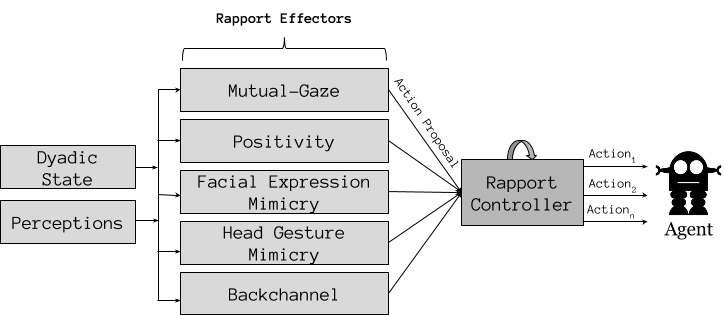
\includegraphics[width=0.48\textwidth]{RapportModel.png}
    \caption{Schematic representation of the rapport model.}
    \label{fig:rapportModel}
\end{figure}

\subsection{Rapport Controller}
\label{sub:sec:modelRapportController}

The \textit{Rapport Controller} manages the proposed actions sent by the different rapport strategies. Each action proposal is a quintuple $A= <G,P,E,I,T>$ containing:

\begin{itemize}
    \item \textbf{Group ($G$)}: part of agent's body that the action is attempting to manipulate;
    \item \textbf{Priority ($P$ where $P \in \mathbb{N}_0$)}: relative importance of the action proposal in relation to others; 
    \item \textbf{Execution description ($E$)}: how the agent will execute the action;
    \item \textbf{Interruption description ($I$)}: how the action should be interrupted by the agent;
    \item \textbf{Timeout ($T$ where $T \in \mathbb{N}$)}: maximum duration.% of the action.
\end{itemize}

Concerning the management of action proposals, the controller periodically captures a snapshot of the agent's ongoing actions and pending action proposals received by the different \textit{Effectors}. Whenever a snapshot is captured or, when receiving a new action proposal, the controller analyses which actions should be interrupted (and replaced). 

\begin{figure}[H]
	\centering
	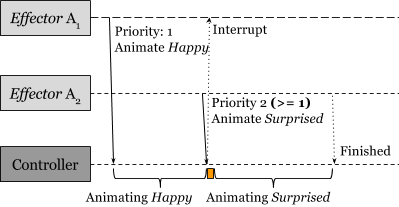
\includegraphics[width=0.38\textwidth]{ConflictingAndInterrupt.png}
	\caption{The action with higher priority interrupts and replaces the action in execution.}	
	%Depiction of an incoming action proposal with different \textit{Group}.
	\label{fig:conflict_interrupt}
\end{figure}

As long as two action proposals, $A$ and $S$, have different groups ($A_G \neq S_G$), both will execute using $A_E$ and $S_E$. However, as illustrated in Figure~\ref{fig:conflict_interrupt}, in the case of a conflict ($A_{1_G}=A_{2_G}$), the action with the highest priority ($A_1$) will interrupt and replace the current one ($A_2$). Moreover, the action can be time limited, therefore, if the action takes longer than expected ($T$) it is interrupted, despite having higher priority. As rule of thumb, idle actions should have a lower priority than actions triggered by discreet states.

\subsection{Stimulate Positivity}

In pursuance of enhancing the first component of rapport, the Positivity rapport\textit{Effector} takes into account the dyadic state of the interaction to trigger vocalisations to motivate, praise, and even humour the interactional partner (Table~\ref{table:positivity_rule_examples}). In addition, the agent should share a personal information to the person (self-disclosure) that plays an important role in closing relationships between two strangers\cite{Kang2011}. 

%The interactional states and the corresponding sentences are specified by the researcher and should tailor to the dyadic state of the interaction as much as possible. For instance, in case of the Portuguese language, which highly inflected on the gender, there have to be distinct sentences for each gender. To conclude, Table~\ref{table:positivity_rule_examples} depicts examples of interactional utterances that the researcher may specify for an agent during a game of Chess.

\begin{table}[H]
	\centering
	\begin{tabular}{|l|l|}
	\hline
	\textbf{Interactional State} & \textbf{Utterance} \\ \hline
	After Introduction & \specialcell{I learnt the castling move today!} \\ \hline
	Player loses the queen & Your king is still well guarded! \\ \hline
	Agent loses a bishop & There goes a bishop! \\ \hline
	\end{tabular}
	\caption{Example utterances depending on the current state of the interaction.}
	\label{table:positivity_rule_examples}
\end{table}

\subsection{Stimulate Mutual Attention}
\label{sub:sec:model_mutual_attention}

Following Figure~\ref{table:BuildingRapportPlan} and~\ref{fig:rapportModel}, the model enhances mutual attention using mutual gaze and backchannel strategies.

The Mutual-Gaze rapport \textit{Effector} bases on the work developed by Andrist et. al.~\cite{Andrist2015}. In short, it swaps between establishing eye contact and looking the game during pre-determined periods of time according to the following conditions: current phase of the scenario (in-task or between-tasks) and the user's personality (introverted or extroverted). The researcher may set the priority of the action proposals, as well as the gaze lengths, which default to the values specified on the work this \textit{Effector} is based on~\cite{Andrist2015}.

The Backchannel \textit{Effector} bases on the work developed by Niewiadomski et. al., on the GRETA system~\cite{Niewiadomski2009} that analyses variations of the pitch to produce listener behaviour. For simplicity, this \textit{Effector} only considers up-down head nods as listener signals. The researcher may set the priority of the generated action proposals, in addition to the trigger probability, the amplitude of the gesture, the gesture velocity, and the number of head nods.

\subsection{Stimulate Coordination}

To enhance coordination, the model uses behavioural mimicry and backchannel strategies.

The Facial Expression Mimicry \textit{Effector} mimics facial expressions (e.g., happiness, surprise, and sadness), triggering animations according to the perceived emotion intensity $I \in \interval{0}{100}$. In addition to the priority of the generated action proposals, the model allows changing the following parameters for each type of emotion: trigger probability, minimum intensity, and priority.

Head Gesture Mimicry \textit{Effector} mirrors head gestures such as up-down nods and left-right shakes ~\cite{Riek2009, Andrist2014, Cassell2007, Wang2009}. In addition to the priority of the generated action proposals, for each gesture, researchers may specify the amplitude, the velocity, and the number of repetitions.

Lastly, the agent should adhere to social norms by, for example, introducing itself when meeting people and saying ``thank you'' when a person does a task for the agent.

%%%%%%%%%%%%%%%%%%%%%%%%%%%%%%%%%%%%%%%%%%%%%%%%%%%%%%%%%%%%%%%%%%%%%%%%%%%%%%%%%%%%%%%%%%

\section{\ac{EMYS}: The Rapport Agent}
\label{sec:model_implementation}

%TODO isto tem potencial para ser cortado
The following section describe the framework that implements the rapport model detailed using \acf{EMYS} robot (Figure~\ref{fig:robots:EMYS2}) as the chosen embodiment to test the rapport agent.

\begin{figure}[H]
	\centering
	\frame{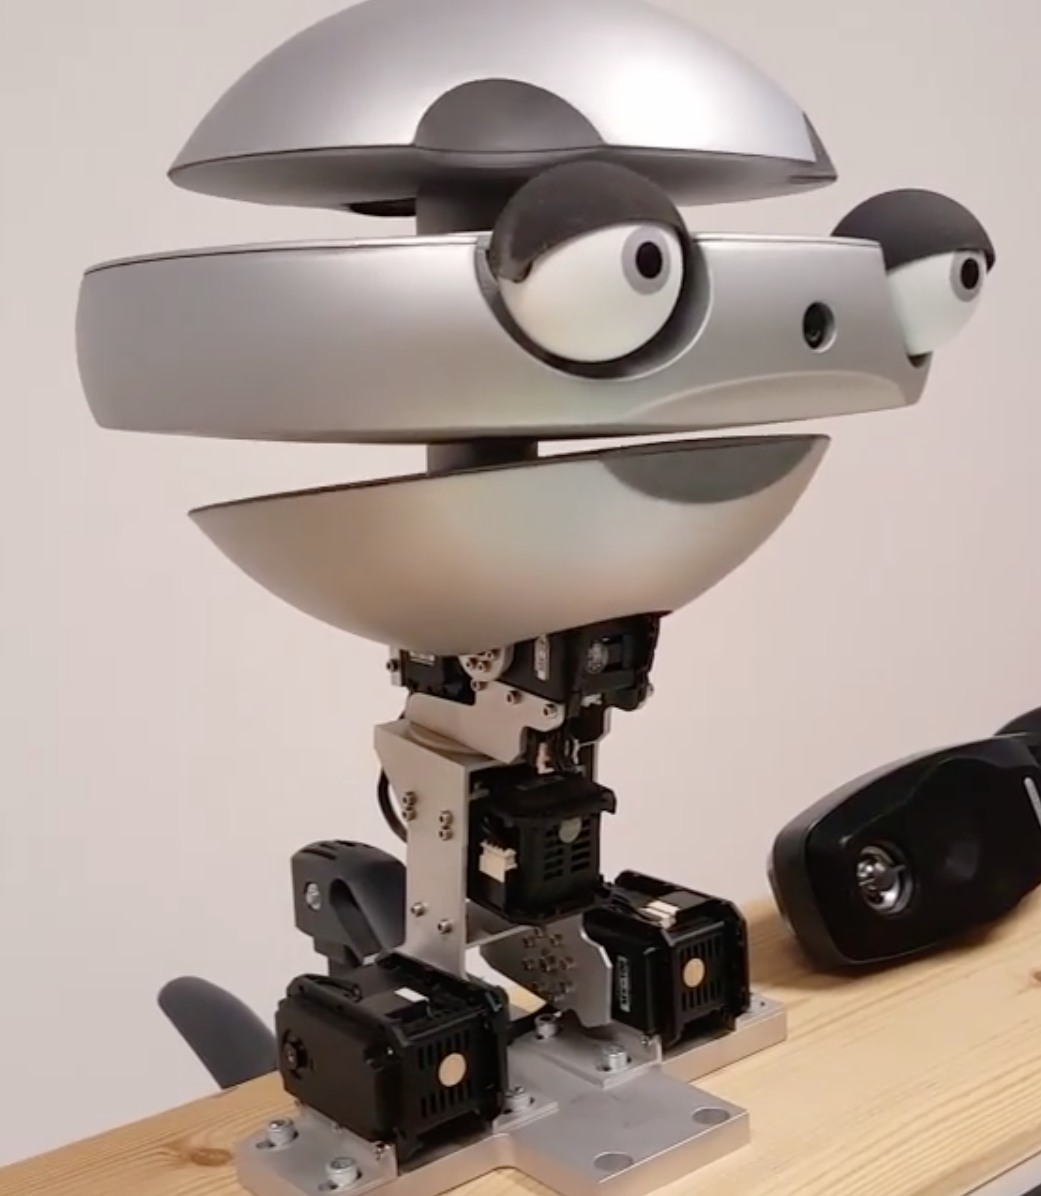
\includegraphics[width=0.1\textwidth]{emys.png}}
	\caption{\ac{EMYS} robot.}
	\label{fig:robots:EMYS2}
\end{figure}

\begin{figure}[H]
	\centering
	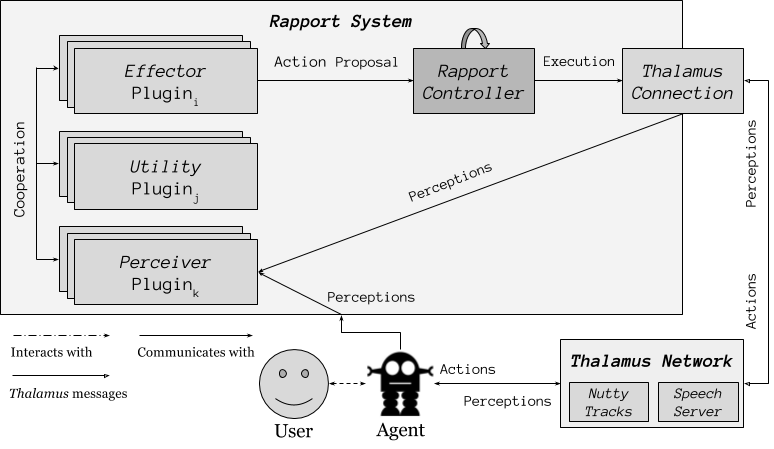
\includegraphics[width=0.47\textwidth]{RapportControllerArchitectureOverview.png}
	\caption{Schematic representation of the framework that implements the rapport model.}
	\label{fig:rapport:archicture}
\end{figure}

The framework follows a plugin-based architecture that, in order to reduce the impact of network delays (Section~\ref{sub:sec:sera}), the internal communication is done using method calls, limiting the number of network messages. Following Figure~\ref{fig:rapport:archicture}, the framework contains the following elements:
\begin{itemize}
	\item \textbf{\textit{Effector Plugins}}: proposes actions and enables/disables plugins;
	\item \textbf{\textit{Perceiver Plugins}}: perceives the external world and informs the interested plugins;
	\item \textbf{\textit{Utility Plugins}}: general purpose plugins that can be used to, for example, store interactional data;
	\item \textbf{\textit{Rapport Controller}}: manages plugins' lifecycle, link plugins, and has the same responsibilities as the rapport model's \textit{Rapport Controller} (Section~\ref{sub:sec:modelRapportController});
	\item \textbf{\textit{Thalamus Connection}}: bridges the system with \ac{SERA}, sending and receiving \textit{Thalamus} messages.
\end{itemize}

The \textit{Cooperation} connection depicted in Figure~\ref{fig:rapport:archicture} establishes the connection between plugins, for example, \textit{Effectors} use \textit{Perceivers} to read perceptual information and may use \textit{Utility} plugins to consult the interaction history. In addition, the \textit{Action} connection is the decisive message that will execute the action proposals defined by the \textit{Effectors} and executed by the \textit{Rapport Controller}.

%The most important connections illustrated in Figure~\ref{fig:rapport:archicture} is 
%Following Figure~\ref{fig:rapport:archicture}, there are five types of connections:
%\begin{itemize}
%	\item \textbf{Perceptions}: perceptual information;
%	\item \textbf{Actions}: the decisive messages that trigger animations or utterances;
%	\item \textbf{Action Proposal}: requests sent by \textit{Effector Plugins};
%	\item \textbf{Execution}: set of actions triggered periodically by the \textit{Rapport Controller} - execution, interruptions or replacement according to the action proposals' stage;
%	\item \textbf{Cooperation}: communication between plugins. For example, for backchannel behaviour, two \textit{Effectors}, one rule-based and one \ac{ML}-based, can cooperate together to trigger the most appropriate social behaviour.
%\end{itemize}


%%%%%%%%%%%%%%%%%%%%%%%%%%%%%%%%%%%%%%%%%%%%%%%%%%%%%%%%%%%%%%%%%%%%%%%%%%%%%%%%%%%%%%%%%%%%%%%%%%

\subsection{Plugins' Lifecycle Management}
\label{sub:sec:pluginLifecycle}

At the startup, the \textit{Rapport Controller} loads the available plugins from a user-selected folder. They are all enabled by default unless specified otherwise through the configuration file that can be accessed using the controller's \ac{GUI} (Figure~\ref{fig:pluginList} in Appendix A). During this process, following Figure~\ref{fig:pluginLifecycle}, each plugin follows a two-step initialisation:

\begin{enumerate}
	\item \textbf{Initialisation}: initialise internal variables;
	\item \textbf{Retrieve Dependencies}: retrieve plugins that it depends on (e.g., \textit{Effectors} typically requires \textit{Perceivers}).
\end{enumerate}

After initialisation, if the \textit{Rapport Controller} is running, \textit{Effectors} can attempt to modify the agent's behaviour concurrently according to the dyadic state of the interaction, until they are disposed of either manually (Figure~\ref{fig:pluginList} in Appendix A), either automatically by another \textit{Effector}. In any case, the plugins are automatically disabled in case of an error without escalating to an application crash.

\begin{figure}[H]
	\centering
	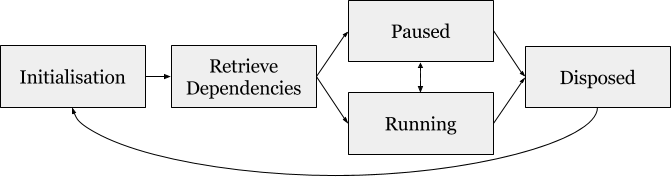
\includegraphics[width=0.47\textwidth]{PluginsLifecycle.png}
	\caption{Plugin's lifecycle.}
	\label{fig:pluginLifecycle}
\end{figure}

\begin{table*}[t]
	\centering
	\begin{tabular}{|l|l|l|l|l|l|}
	\hline
	\multicolumn{1}{|c|}{\textbf{Category}} & \multicolumn{1}{c|}{\textbf{Subcategory}} & \textbf{Utterance}                                                                                      & \textbf{Priority} & \textbf{Delay (ms)} & \textbf{Timeout (ms)} \\ \hline	
	intro & greet & \specialcell{Hi! $<$gaze(person)$>$} I'm EMYS! & 2 & 0 & 30000 \\ \hline
	game & score & \specialcell{Yey! $<$Animate(surprise2, 3)$>$} & 2 & 0 & 30000 \\ \hline
	game & results & \specialcell{Managed $|$\texttt{Points}$|$!\\$<$gaze(person, 3, 500, 5000)$>$} & 2 & 0 & 30000 \\ \hline
	end & ending & \specialcell{Thank you for your participation!\\$<$animate(happy4, 4, 1000)$>$} & 3 & 0 & 30000 \\ \hline		
	\end{tabular}
	\caption{Example compilation of utterances compatible with the developed system. Actions are delimited by $<$ and $>$, and substitution variables by $|$.}
	\label{fig:extended:utterances}
\end{table*}


\subsection{Managing Actions}
\label{sub:sec:managingActions}

The \textit{Rapport Controller} manages action proposals as described in Section~\ref{sub:rapportModel}. However, in addition to the elements of action proposal quintuple $A=<G,P,E,I,T>$, the controller stores the following information:
\begin{itemize}
	\item \textbf{Status}: \textit{pending}, \textit{executing}, \textit{executed} or \textit{interrupted};
	\item \textbf{Starting time}: when the action has started executing; %TODO potential candidate to compact
	\item \textbf{\textit{Thalamus} identifier}: to monitor when actions have finished by monitoring the \textit{Thalamus} messages sent by \textit{Nutty Tracks} and \textit{Speech Server}.
\end{itemize}

The status field is required to manage the state of each action proposal. For example, following Figure~\ref{fig:actionProposalStatus}, an action proposal is only interrupted (using $I$) if its previous state was \textit{executing}. In the absence of the \textit{Thalamus} identifier, we could not flag the actions as executed, making them transition automatically to the \textit{interrupted} state.

\begin{figure}[H]
	\centering
	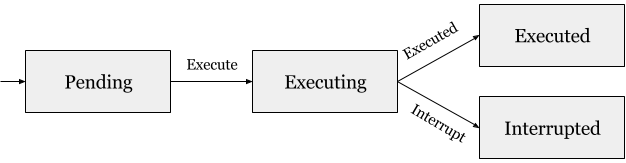
\includegraphics[width=0.47\textwidth]{ActionProposalCycle.png}
	\caption{Action Proposal available states and the corresponding transition graph.}
	\label{fig:actionProposalStatus}
\end{figure}

To conclude, the execution and the interruption descriptions of the action proposal ($E$ and $I$, respectively) are self-contained functions specified by the researcher, therefore they can contain additional logic. However, they must at least send the required \textit{Thalamus} messages to either \textit{Nutty Tracks} or \textit{Speech Server} to produce animations or utterances, respectively.

%%%%%%%%%%%%%%%%%%%%%%%%%%%%%%%%%%%%%%%%%%%%%%%%%%%%%%%%%%%%%%%%%%%%%%%%%%%%%%%%%%%%%%%%%%%%%%%%%%%%%%%%%%%%%%%%%%%%%%%%%%%%%%%%%%%%%%%%%%%%%%%%%%%%%%%%%%%%%%%%%%%%%%%%%%%%%%%%%%%%%%%%%%%%%%%%%%%%%%%%%%

\section{Plugins}
\label{sec:plugins}

There are three types of plugins: \textit{Effectors}, \textit{Perceivers}, and \textit{Utility}. Transparently to the developer, each plugin may specify its \ac{GUI}, and more, importantly, its configuration file (e.g., Listing~\ref{lst:MimicFacialExpressionsSettings}) that allows researchers to tailor the agent's behaviour to the interactional goals of the scenario without having to recompile the code.

%TODO se precisar de espaço, posso tentar compactar isto

\begin{lstlisting}[caption={Excerpt of the \ac{XML} configuration file used by Mimic Facial Expressions \textit{Effector}.}, label={lst:MimicFacialExpressionsSettings},language=XML]
<MimicFacialExpressionsSettings>
  <MinimumMimicDelay>3500</MinimumMimicDelay>
  <Happy>
    <Probability>0.5</Probability>
    <MinimumIntensity>0.65</MinimumIntensity>
    <Priority>1</Priority>
    <BaseAnimation>sadness</BaseAnimation>
  </Happy>
</MimicFacialExpressionsSettings>
\end{lstlisting}

Researchers may additional define a high-level \textit{Effector} that is capable of deactivating and enabling other plugins in runtime, giving the agent the ability to map the rapport strategies to discreet states of the scenario.

We also noticed that some \textit{Effectors} frequently interrupt themselves repeatedly. To solve this issue, we added, transparently to the developer, a mechanism to track internally the proposed actions by specifying the minimum delay between each action proposals. The researcher can choose on of the following levels:

\begin{itemize}
	\item \textbf{Unrestricted}: the \textit{Effector} must explicitly manage its proposed actions;
	\item \textbf{One Action Globally}: the \textit{Effector} cannot interrupt itself unless with a proposal with higher priority;
	\item \textbf{One Action Per Group}: same as \textit{One Action Globally} but with granular to the \textit{Group}.
\end{itemize}

\subsection{Agent Actions Manager}
\label{sub:sec:agentActionsManager}

%Mencionar que é este o plugin que tem a Thalamus Connection para executar acções

The Agent Actions Manager is a \textit{Utility} plugin with the following goals:
\begin{itemize}
	\item Monitors agent's actions to notify the controller;
	\item Provide convenient wrappers for common action proposals, describing both $E$ and $I$;
	\item Provide non-technical researchers with the tools to change the agent's behaviour without worrying about implementation details.
\end{itemize}

The first objective is achieved by monitoring the messages that \ac{SERA} sends to the \textit{Thalamus Network}. The second objective aims to reduce the amount of code required to specify common action proposals. To accomplish the last goal, similar to \textit{Skene}, this plugin provides a \ac{GUI} (Figure~\ref{fig:agentActionsManagerScreenshot} in Appendix A) to change the agent's behavioural rules (utterances) using mark-up text (Table~\ref{fig:extended:utterances}). Taking advantage of the rapport model, following Expression~\ref{eq:behaviour}, these utterances may contain interruptible or time-limited actions with different priorities.

\begin{equation}
	<action(arg_1, arg_2, ..., arg_n, [priority], [delay], [timeout])>
	\label{eq:behaviour}
\end{equation}

%%%%%%%%%%%%%%%%%%%%%%%%%%%%%%%%%%%%%%%%%%%%%%%%%%%%%%%%%%%%%%%%%%%%%%%%%%%%%%%%%%%%%%%%%%%%%%%%%%%%%%%%%%%%%%%%%%%%%%%%%%%%%%%%%%%%%%%%%%%%%%%%%%%%%%%%%%%%%%%%%%%%%%%%%%%%%%%%

\section{Effectors Implementation}

The following section describes the technologies that supports the rapport \textit{Effectors}, their parametrisation and the encountered issues. 

The Positivity rapport \textit{Effector} (that satisfies the ``Stimulate positivity'' goal) and the ``Adhere to Social Norms'' goal are implemented by triggering utterances given the perceptual information of the scenario. 

\subsection{Supporting Technologies}

Revisiting the rapport model described in Section~\ref{sub:rapportModel}, the rapport \textit{Effectors} needs to monitor the dyadic state and perceive the user's emotion, speech disfluencies and head gestures. To this end, following Figure~\ref{fig:SupportingTechnologiesOverview} there are four main components to support the rapport strategies:
\begin{itemize}
	\item \textbf{\ac{SSI}}: framework to recognise social signals in realtime~\footnote{\url{http://hcm-lab.de/projects/ssi/}}~\cite{Wagner2013};
	\item \textbf{SHORE}: recognise facial features from a video feed~\cite{Ruf2011};
	\item \textbf{openSMILE}: extracts prosody features~\cite{Eyben:2013:RDO:2502081.2502224};
	\item \textbf{GRETA\textsuperscript{PP}}: adapted version of GRETA~\cite{Niewiadomski2009} to generate listener behaviour and redirect perceptions;
	\item \textbf{GRETA \textit{Perceiver} Plugin}: proxy between GRETA\textsuperscript{PP} and the \textit{Rapport Controller}.
\end{itemize}

\begin{figure}[H]
	\centering
	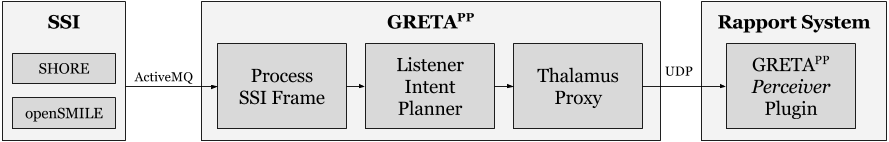
\includegraphics[width=0.47\textwidth]{figures/SupportingTechnologiesOverview.png}
	\caption{Schematic representation of the components that supports the rapport model.}
	\label{fig:SupportingTechnologiesOverview}
\end{figure}

GRETA\textsuperscript{PP} is a variation of the GRETA system~\cite{Niewiadomski2009} that contains solely its \textit{Listener Intention Planner} rule-based component that behaves identically to the rapport model's \textit{Backchannel} \textit{Effector}. The perceptions and the generated behaviour are sent to the GRETA\textsuperscript{PP} \textit{Perceiver} Plugin using \ac{UDP} sockets so that it notifies the interested \textit{Effectors}. The system has a slight delay ($<$ 1 second), as the refresh rate had to be halved to 5Hz so that the system could handle the resource heavy \ac{SSI}.

The following \textit{Effectors}' parameters were parametrised empirically following several pilots on 3 different people. The generated action proposals have the priority of 1, with the exception of Backchannel \textit{Effector} that has priority of 2 as it is not considered an idle behaviour. Finally, the mimicry behaviour is only done once every 3500ms.

%%%%%%%%%%%%%%%%%%%%%%%%%%%%%%%%%%%%%%%%%%%%%%%%%%%%%%%%%%%%%%%%%%%%%%%%%%%%%%%%%%%%%%%%%%%%

\subsection{Facial Expression Mimicry}
\label{sub:sec:facialExpressionMimicryImplementation}

The Facial Expression Mimicry rapport \textit{Effector} mimics the user's emotion given SHORE's emotion with highest intensity. With the probability of 50\%, it proposes actions, as long as happiness, sadness, and anger intensities detected are 0.65, 0.65, and 0.5, respectively. Nonetheless, the implementation of this plugin is not without issues as SHORE was detecting happy emotions in absence of faces. We solved that issue by applying a smoothing signal at the cost of increasing the delay from less than 1 second, to at most 3 seconds. In the end, we opted to remove the smoothing filter and compensate with disabling it when the user was not present.

%TODO nao estou a falar das animacoes aleatorias

\subsection{Head Gestures Mimicry}

The Head Nod Mimicry \textit{Effector} proposes up-down nod gestures and left-right head shakes given Kinect's perceived head gesture. As the sensors seldom detected head gestures during the pilot tests, both gestures' probabilities are set to 1. In addition, it produces light head nods that are slightly randomised in each action proposal to avoid being repetitive.

\subsection{Mutual-Gaze}
The Mutual-Gaze \textit{Effector} swaps the gaze target depending on the current state of the interaction assuming that the user is extroverted (lowest standard deviation), as we are unable to know the personality beforehand. The gaze durations are the default values.

\subsection{Backchannel}
The Backchannel \textit{Effector} produces listener behaviour according to the GRETA system~\cite{Niewiadomski2009}, proposing up-down head nods actions.  However, we were unable to reduce the impact of noise (agent's robotic movement and voice) on the \ac{SSI} sensors, leading to excessive false positives. Despite the attempts of counteracting the issue through noise-suppressing directional microphones and adjusting the sensors' parameters, the issue persisted, therefore the Backchannel \textit{Effector} was not used during the studies.